% !TEX root = main.tex
Today's complex cyber-physical systems are characterized by the interaction of a large number of heterogeneous components. Consequently, the models used to analyze these systems are equally complex and consist of heterogeneous sub-models relying on different assumptions and based on principles from different scientific disciplines. It is not uncommon to encounter a patchwork of differential equations, difference equations, hybrid automata, lookup tables, custom switching logic, low-level legacy code, etc. To further compound the difficulty in analyzing these systems, different components of a complex engineered system are typically designed by different suppliers. Although a high-level specification for these components may be known, detailed models are not available for intellectual property reasons. We are thus faced with a tremendous gap between the existing analysis techniques that rely on closed-form models and the models available in industry. It is, therefore, not surprising the emphasis that industry places on simulation since despite the complexity of models, it is always possible to simulate them. This raises the question of whether we can provide formal guarantees about certain properties of these complex systems based solely on the information obtained via their simulations. In this paper, we focus on one of the most important of such properties in the context of control theory: stability.

More formally, we consider a dynamical system as in:
\vspace{-0.88394mm}
\begin{equation}\label{eq:dynamicalsystemGeneral}x_{k+1} = f(k, x_k),
\end{equation}
where, $x_k \in X$ is the state and $k \in \N$ is the time index. In this paper, we focus on switched systems, but we believe that the presented results can be extended to more general classes of dynamical systems.
We start with the following question to serve as a stepping stone: For some $l \in \N_{>0}$, given $N$ traces of length $l$, $(x_0^1,x_1^1,\dots, x_l^1)$, $(x_0^2,x_1^2,\dots, x_l^2)$, $\ldots$, $(x_0^N,x_1^N,\dots,x_l^N)$ belonging to the behavior of the system \eqref{eq:dynamicalsystemGeneral}, (i.e., $x_{k+1}^i = f(k, x_k^i)$ for any $k \in \{0,\dots,l-1\}$ and any $i \in \{1,\dots,N\}$), what can we say about the stability of the system \eqref{eq:dynamicalsystemGeneral}? For the rest of the paper, we use the term \emph{black-box} to refer to models where we do not have access to the model, i.e., to $f$, yet we can indirectly learn information about $f$ by observing traces of length $l$ (becoming, in the particular case where $l=1$, couples of points $(x_k, y_k)$ as defined in \eqref{eq:dynamicalsystemGeneral}).
%\textcolor{red}{We should say that this is non-ideal when we don't know what the state is, but it is a start, and it makes sense in certain situations. Paulo's comment: If we don't have a model, then we don't know what the state is. But the issue I raised is even deeper. Why can we assume that we can initialize the state randomly? Joris' comment: we do not necessarily assume that WE initialize the set randomly. We have random observations of the state, we do not know the process that picks the state, and we model this process with a random distribution. By default we take it uniform since we cannot say some states are privileged a priori. But a future step would be to consider different distributions and extend our guarantees to them.}

A potential approach to this problem is to first identify the dynamics, i.e., the function $f$, and then apply existing techniques from the model-based stability analysis literature. However, unless $f$ is a linear function, there are two main reasons behind our quest to directly work on system behaviors and bypass the identification phase: 1) Even when the function $f$ is known, in general, stability analysis is a very difficult problem \cite{stabilityHard1}; 2) Identification can potentially introduce approximation errors, and can be algorithmically hard as well. Again, this is the case for switched systems \cite{lauer}. A fortiori, the combination of these two steps in an efficient and robust way seems far from obvious.

In recent years, increasing number of researchers started addressing various verification and design problems in control of black-box systems \cite{bianchini, balkan, mitra, mitra2}. In particular, the initial idea behind this paper was influenced by the recent efforts in \cite{topcu, kapinski}, and \cite{lazar} on using simulation traces to find Lyapunov functions for systems with known dynamics. In these works, the main idea is that if one can construct a Lyapunov function candidate decreasing along several finite trajectories starting from different initial conditions, it should also decrease along every other trajectory. Then, once a Lyapunov function candidate is constructed, this intuition is put to test by verifying the candidate function either via off-the-shelf tools as in \cite{topcu} and \cite{kapinski}, or via sampling-based techniques as in \cite{lazar}. This also relates to almost-Lyapunov functions introduced in \cite{liberzon}, which presents a relaxed notion of stability proved via Lyapunov functions decreasing everywhere except on a small set. Note that, since we do not have access to the dynamics, these approaches cannot be directly applied to black-box systems. However, these ideas raise the following problem that we address in this paper: By observing that a candidate Lyapunov function decreases on a large number of observations, we empirically build a certain confidence that such candidate Lyapunov function is a bona-fide Lyapunov function. \emph{Can we translate this confidence into a confidence that this Lyapunov function decreases at most of the points in the state space?} 

Note that, even in the case of a 2D linear system, the connection between these two beliefs is nontrivial. In fact, one can easily construct an example where a candidate Lyapunov function decreases everywhere on its levels sets, except for an arbitrarily small subset, yet, almost all trajectories diverge to infinity. For example, the system
\[
x^+ = \begin{bmatrix}
0.14 & 0\\
0 & 1.35
\end{bmatrix}x,
\]
admits a Lyapunov function candidate on the unit circle except on the two red areas shown in Fig. \ref{fig:levelset}.
Moreover, the size of this ``violating set" can be made arbitrarily small by changing the magnitude of the unstable eigenvalue. Nevertheless, the only trajectories that do not diverge to infinity are those starting on the stable eigenspace that has zero measure.
\begin{figure}
\begin{center}
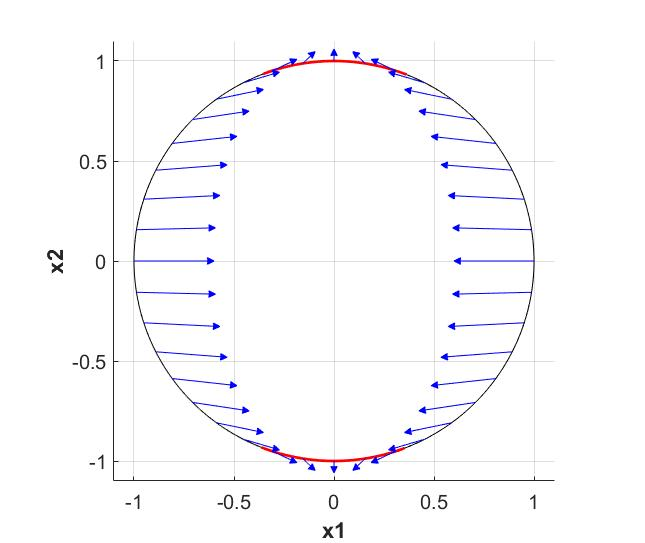
\includegraphics[trim = 15mm 15mm 10mm 10mm, scale=0.3]{ex1.jpg}
\end{center}
\caption{A simple dynamics and the level set of an ``almost Lyapunov function''. Even though this function decreases at almost all points in its level set, almost all trajectories diverge to infinity.}
\label{fig:levelset}
\end{figure}

In this paper, we take the first steps to infer stability from observations of switched linear systems. In addition to the preceding example, there are other reasons to temper our expectations for proving stability from data: identifying and deciding stability from of arbitrary switched linear systems is NP-hard \cite{jungers_lncis}.

The stability of switched systems is closely related to the \emph{joint spectral radius} (JSR) of the matrices modeling the dynamics in each mode. Deciding stability amounts to deciding whether the JSR is less than one \cite{jungers_lncis}. In this paper, we present an algorithm to bound the JSR of a switched linear system from a finite number $N$ of observations. This algorithm partly relies on tools from the random convex optimization literature (also known as chance-constrained optimization, see \cite{campi,nemirovski,campi-garatti}), and provides an upper bound on the JSR with a user-defined confidence level. As $N$ increases, this bound gets tighter. Moreover, with a closed form expression, we characterize what is the exact trade-off between the tightness of this bound and the number of samples. In order to understand the quality of our upper bound, the algorithm also provides a deterministic lower bound. Finally, we provide an asymptotic guarantee on the gap between the upper and the lower bound, for large $N$.

%\textcolor{blue}{We note that, aside from the stability analysis, black-box setting has been adopted by several researchers in the analysis and control of dynamical systems in the recent years. For example, in \cite{bianchini}, the authors consider the tuning a black-box plant by choosing suitable inputs. In \cite{balkan}, by exciting a black-box system with different inputs, authors generate test cases to challenge the system with respect to a given design specification.} \textcolor{red}{Anything more here?}

The organization of the paper is as follows: In Section \ref{sec:preliminaries}, we introduce the notations and provide the necessary background in stability of switched systems. In Section \ref{sec:lowerbound}, we present a deterministic lower bound for the JSR. Section \ref{sec:upperbound} presents the main
contribution of this paper where we provide a probabilistic stability guarantee for a given switched system, based on finite observations. We experimentally demonstrate the performance of the presented techniques in Section \ref{sec:experiments} and conclude in Section \ref{sec:conclusions}, while hinting at our related future work.
%. Topcu et.al. \cite{topcu}, Kapinski et.al. \cite{kapinski}construct Lyapunov function candidates using the simulation traces, however to be able to formally verify the constructed Lyapunov function, they require the knowledge of the full dynamics. In \cite{lazar} and \cite{lazar2} Bobiti and Lazar address this and provide sampling based probabilistic and deterministic guarantees of a given Lyapunov function candidate.

% The answer is immediate when \eqref{eq:dynamicalsystemGeneral} is a linear time-invariant system because we can simply identify $f$ by $n$ linearly independent output trajectories.  



%In this paper, we seek the answer to this question for switched linear systems for which the problem immediately becomes nontrivial. A switched linear systems is in the form:
%\begin{equation}\label{eq:switchedSystem}x_{k+1} = A_{\sigma(k)}x_k,\end{equation}
%where, $\sigma: \N \to \{1,2, \ldots, m\}$ is the switching sequence and $A_{\sigma(k)} \in \calM$, for all $\sigma$ and $k$. Aside from their theoretical value, switched systems model the behavior of dynamical systems in the presence of known or unknown varying parameters. These parameters can model internal properties of the dynamical system such as uncertainties, look-up tables, values in a discrete register as well as exogenous inputs provided by a controller in a closed-loop control system. 

%\textcolor{red}{There is no model.
%System are getting more complex, multimodal, lookup tables, thermodynamics, there is a need to ?prove properties about these systems, despite the fact that the modesl are mo complex are partially knowni Subcomponetns come from  different companies and black box.
%We still need to prove properties.
%The most important property in terms of control: stability.
%Even in the case when we have a model the stability is hard, for example Raphael, therefore we shouldn't expect we are gonna do better. The first step towards just based on switched systems. Because these are the very simple class of systems, resoanable it captures many applications.
%Even in the case of linear systems we cannot say anything. Here, we put the example where even the system is linear, we cannot say anything by just looking at the lyapunov functions decrease.}


%To make our reasoning clearer, we introduce the \emph{Lyapunov exponent} of the system \eqref{eq:switchedSystem}, which is a numerical quantity describing its stability.
%\begin{definition} Given a dynamical system as in \eqref{eq:dynamicalsystem} its \emph{Lyapunov exponent} is given by
%$$\rho =\inf{\{r:\,\forall x_0, \exists C\in \re^+: \quad x(0)=x_0 \Rightarrow x(t)\leq Cr^t\}}. $$
%\end{definition}
%Under certain conditions, deciding stability amounts to decide whether $\rho<1.$  In order to understand the quality of our techniques, we will actually try to prove lower and upper bounds on $\rho.$ 
%Assessing the stability of nonlinear systems by leveraging simulations has been an active area of research in the recent years. Simulation data has been used in both construction and verification of Lyapunov functions. Topcu et.al. \cite{topcu} and Kapinski et.al. \cite{kapinski} construct Lyapunov function candidates using the simulation traces, however to be able to formally verify the constructed Lyapunov function, they require the knowledge of the full dynamics. In \cite{lazar} and \cite{lazar2} Bobiti and Lazar address this and provide sampling based probabilistic and deterministic guarantees of a given Lyapunov function candidate. The presented method requires the knowledge of how fast the output of the system can change as the initial condition changes, and moreover the number of required samples increases exponentially in the dimension of the state, $n$.

%The stability of switched systems closely relates closely to the \emph{joint spectral radius} (JSR) of the matrices appearing in \eqref{eq:switchedSystem}. Under certain conditions deciding stability amounts to deciding whether JSR less than one or not. There has been a lot of work on developing algorithms to approximate this quantity, when the matrices appearing in \eqref{eq:switchedSystem} are known. Therefore, our work is also connected to the identification of switched systems, since once the system \eqref{eq:switchedSystem} is identified one can then apply these well-established results. However, there are two main reasons behind our quest to directly work on input-output pairs and bypassing the identification phase: (1) Even when $\calM$ is known, approximating the JSR is NP-hard \cite{jungers}. (2) Identifying the set $\calM$ is also NP-hard. Therefore, the existing identification techniques can identify $\calM$ up to an approximation error. As a result, how to relate this identification error to an error on the stability of \eqref{eq:switchedSystem} is still nontrivial.

%In this paper, we present an algorithm to approximate the JSR of a switched linear system from $N$ input-output pairs. This algorithm provides an upper bound on the JSR with a user-defined confidence level. As the number of samples increases, this bound gets tight. Moreover, we characterize with a closed form expression what the exact trade-off between the tightness of this bound and the number of samples is. In order to understand the quality of our technique, the algorithm also provides a deterministic lower-bound.

%The organization of the paper is follows: Section \label{preliminaries} introduces our notation and definitions from the switched linear system literature to present our results, Section \label{problemDefinition} formalizes the problem definition, Section \label{upperBound} provides an algorithm to compute a deterministic lower bound and 
%
%In this paper, we consider discrete-time switched linear systems of the form:
%\begin{equation}\label{eq:dynamicalsystem}x_{k+1} = A_{\sigma(k)}x_k,
%\end{equation}
%where, $x_k \in \R^n$, k is index of time and $\sigma: \N \to \{1,2, \ldots, m\}$ is the switching sequence. Let $y_k := x_{k+1}$. 
%We ask the following question:
%\begin{centering}
%\emph{Given N input-output-matrix pairs, $(x_1, y_1)$, $(x_2, y_2)$, $\ldots$, $(x_N, y_N)$ such that
%\begin{equation}\label{eq:triples}y_{k} = A_{\sigma(k)}x_k,
%\end{equation} for some $\sigma(k),$ what can we say about the stability of the system \eqref{eq:dynamicalsystem}?
%\end{centering}
%The only instance where answer to this question has been clearly shown is for linear time-invariant systems.
%
%Note that if \eqref{eq:dynamicalsystem} is a linear time-invariant system with only one mode, this question is easily answered by observing $n$ linearly independent data points. Switched systems can be used to model the behavior of a system of interest for different values of a parameter that varies. This parameter can represent internal parameters such as model uncertainties, as well as exogenous parameters such as inputs provided by a controller in a closed-loop control system. 


%- Stability analysis of dynamical systems is a challenging task. \\
%- Most methods in literature rely on knowing the model. Cite \\
%- How to make the case about the assumption of switched linear yet, we don't construct a model? Here cite
%something that says that this is a hard problem in general. (What is the relationship between switching linear regression)
%- Here we present stability analysis from data, this is easy for linear systems. We present something for switch linear.



%I can refer to the condition number paper?
